% This is a template for BU-ECE Technical Report.
%
% Depending on report content and author preference, a BU-ECE report may be
% in one of the two following styles:
%
%   - genuine report based on ``report'' style, i.e., with chapters, much like
%     a thesis; can be single- or double-sided,
%
%   - report based on ``article'' style, i.e., with no chapters (only sections,
%     subsections, etc.), much like a journal or conference paper; can be
%     single- or double-sided.

% =====================================================================

%\documentclass[12pt]{report}          %Single-sided report style (chapters)
%\documentclass[12pt,twoside]{report}  %Double-sided report style (chapters)
%\documentclass[12pt]{article}         %Single-sided article style (no chapters)
\documentclass[12pt,twoside]{article} %Double-sided article style (no chapters)

\usepackage{bu_ece_report}
\usepackage[utf8]{inputenc}
\usepackage[spanish]{babel}
\usepackage{amsmath}
\usepackage{amsfonts}
\usepackage{amssymb}
\usepackage{makeidx}
\usepackage{graphicx}
\usepackage{lmodern}
\usepackage{float}
\usepackage{hyperref}

% In case an adjustment of vertical or horizontal margins is needed
% due to particular LaTeX/dvips or OS installation, you can uncomment
% and edit the following definitions.
% -------------------------------------------------------------------
%\topmargin       0.00 in
%\oddsidemargin   0.50 in
%\evensidemargin  0.00 in

\begin{document}

% Definitions.
% ------------
\buecedefinitions%
        {SEGUROS DE SALUD TRAS LA PANDEMIA: MEDIR LA TRANSFORMACIÓN}
        {SEGUROS DE SALUD TRAS LA PANDEMIA. INFORME 2}
        {David Moriña, Amanda Fernández-Fontelo y Montserrat Guillén}
        {Octubre 2022}
        {YYYY-NN} % Number of the report (four year digits and number)

% Box with title to fit the opening in the cover
% (adds an empty page in double-sided printing mode).
% ---------------------------------------------------
\buecereporttitleboxpage

% Title page
% (adds an empty page in double-sided printing mode).
% ---------------------------------------------------
\buecereporttitlepage

% Special page, e.g., if the report is restricted or
% to whom it is dedicated, etc., otherwise skip.
% (adds an empty page in double-sided printing mode).
% ---------------------------------------------------
%\bueceprefacepage{Here comes a special preface page. For example, if the report
%is restricted, then a suitable note can be included. This page can also be used
%to indicate to whom the document is dedicated, etc.}

% Report summary; max. 1 page.
% (adds an empty page in double-sided printing mode).
% ---------------------------------------------------
\pagenumbering{roman}
\setcounter{page}{1}
\buecereportsummary{Los confinamientos y otras medidas de restricción de la movilidad adoptadas por muchos gobiernos de todo el mundo para minimizar el impacto de la pandemia de Covid-19 en curso provocaron un descenso en la utilización de los servicios de los seguros de salud públicos y privados por parte de los asegurados y una transformación de la interacción entre los pacientes y el personal sanitario, con una mayor preferencia por la consulta telefónica. Existe una reciente preocupación por determinar si, por efecto del aplazamiento de las visitas o por las secuelas de haber sufrido el virus (Covid-19 persistente o efectos secundarios), se producirá un exceso de uso en los próximos meses, especialmente en diagnósticos graves como el cáncer y entre subpoblaciones vulnerables como las personas mayores.
En este informe se recogen los impactos de la pandemia de Covid-19 en el uso de servicios sanitarios ya descritos en la literatura, y se incluyen los resultados preliminares del análisis del rendimiento del modelo matemático propuesto para analizar este fenómeno mediante un exhaustivo estudio de simulación. Parte del contenido de este informe se ha publicado recientemente en el Boletín de la Sociedad de Estadística e Investigación Operativa (BEIO), y se puede consultar en \url{https://www.seio.es/wp-content/uploads/2022/07/Julio2022_Estadistica.pdf}.} %LA IDEA ÉS DEDICAR EL DARRER INFORME A LES ANÀLISIS DE LES DADES DE MAPFRE EXCLUSIVAMENT. DESPRÉS FALTARÀ UN INFORME GLOBAL, QUE ENTENC SERÀ LA UNIÓ/RESUM DELS ALTRES TRES.

% Table of contents, list of figures and list of tables.
% ``\bueceemptypage'' adds empty page in double-sided
% printing mode and performs ``\clearpage'' in single-sided
% mode.
% ------------------------------------------------------
\tableofcontents\bueceemptypage
\listoffigures\bueceemptypage
\listoftables\bueceemptypage

% Switch on running headers for the report:
%   odd pages  - title (lowercase); if too long, use
%                the first few words followed by ``...'',
%   even pages - last names of the authors.
% -------------------------------------------------------
\buecereportheaders

% Introduction.
% -------------
\pagenumbering{arabic}
\setcounter{page}{1}

\section{Introducción}  % Article style
Existe una enorme preocupación mundial en torno a la infección por el coronavirus aprecido en 2019 (SARS-CoV-2)
en los últimos años, lo que llevó a la Organización Mundial de la Salud (OMS) a declarar
emergencia de salud pública a principios de 2020. Las consecuencias derivadas de la pandemia
causadas por este virus han tenido un profundo efecto en muchas áreas de la actividad humana. En
además de las consecuencias directas en relación a las muertes provocadas por la enfermedad Covid-19
y la saturación de los sistemas de salud en muchos países (incluyendo España y vecinos
países), en 2020 se ha detectado una disminución en el uso de los servicios de salud, tanto
de los propios del Sistema Sanitario Público como de servicios asociados a seguros privados de salud. Muchas personas no han recibido o han retrasado la atención que necesitaban, como vacunas o intervenciones contra el cáncer para prolongar la vida (\cite{baum_admissions_2020, mcdonald_early_2020, maringe_impact_2020}). Según una encuesta de la OMS, este problema con respecto a los servicios de atención médica es especialmente grave entre los países de bajos ingresos (\cite{noauthor_pulse_nodate}), y hay estimaciones de que la reducción de las intervenciones esenciales de salud maternoinfantil puede causar más de un millón de muertes infantiles adicionales (\cite{roberton_early_2020}). 

La investigación del impacto de los cambios en la utilización de la asistencia sanitaria en los resultados y costes sanitarios presenta importantes desafíos metodológicos. La carga real de Covid-19, en primer lugar, no se puede estimar fácilmente, teniendo en cuenta que muchos casos cursan de forma asintomática o con síntomas leves y no se registran en las fuentes oficiales. Varios enfoques metodológicos han sido propuestos recientemente en la literatura; por ejemplo, la incidencia real de Covid-19 en España ha sido estimada utilizando diferentes métodos en \cite{fernandez-fontelo_estimating_2020, morina_cumulated_2021}, lo que lleva a la conclusión de que aproximadamente entre el 25\% y el 40\% de los casos reales no se notificaron.

La primera disminución en la utilización de los servicios de salud debido a las consecuencias de la pandemia de Covid-19 se observó en China en febrero de 2020, tras varios meses de tendencia creciente. Mediante un análisis de series temporales (2016-2020), en \cite{xiao_impact_2021} los autores cuantifican la disminución en febrero de 2020 hasta en un 63\% (95\% intervalo de confianza: 61\%-65\%) en consultas por cualquier causa en hospitales de regiones con alto Índice de Desarrollo Humano (IDH).

Una revisión sistemática publicada recientemente basada en 81 artículos (\cite{moynihan_impact_2021}) de muchos países con circunstancias sociopolíticas y económicas muy diferentes revela que, aunque la mayoría de los servicios de salud experimentaron una disminución en su uso (95.1\% de los servicios considerados), algunos servicios registraron un incremento (la mayoría relacionados con servicios telemáticos o telefónicos). El cambio porcentual osciló entre un aumento del 49\% y una disminución del 87\% con una reducción mediana del 37.2\% (IQR -50.5\% a -19.8\%). Este estudio también muestra que los cambios más significativos se observaron entre mediados de febrero y fines de mayo de 2020, cuando se aplicaron las medidas no farmacéuticas más restrictivas en la mayoría de los países.

También se ha estudiado el impacto de estos cambios en la utilización de los servicios de salud en la salud mental de los pacientes, y se ha encontrado que son especialmente significativos entre las poblaciones vulnerables. En este sentido, en \cite{bastani_factors_2021} los autores identifican la salud mental y los servicios de salud digital como problemas importantes que influyen o contribuyen a la salud de las personas mayores durante la pandemia de Covid-19.

\subsection{Retraso en los diagnósticos}\label{sec:diagnoses}
Un retraso en obtener un diagnóstico puede tener consecuencias importantes en la salud del paciente y, en algunos casos, en las probabilidades de supervivencia. Sin embargo, se sabe que las medidas no farmacéuticas del Covid-19 llevaron a una reducción en el número de diagnósticos debido al cierre de los servicios de salud y las restricciones de movilidad, lo que probablemente produzca un número sin precedentes de retrasos en los diagnósticos. Según \cite{moynihan_impact_2021}, sin desagregar por servicio ni diagnóstico, se puede observar que el porcentaje de reducción osciló entre el 10\% y el 85\%, con una mediana de reducción del 31,4\% (RIC -52,5\% a -23,8\%). Se observaron valores similares en cuanto a los cambios en la atención terapéutica y preventiva (29,6\% de reducción mediana con IQR -56,8\% a -19,2\%), aunque ya se observaba una tendencia creciente a fines de abril de 2020. Al considerar por separado según la gravedad de la enfermedad del usuario del servicio, se observó un patrón de mayores reducciones entre aquellos con enfermedades más leves o menos graves en comparación con aquellos con enfermedades más graves en casi la mitad de los resultados considerados, mientras que para la otra mitad no se observaron diferencias y ninguno de los estudios incluidos en la revisión informaron una reducción más pequeña entre aquellos con una enfermedad más leve o menos grave.

La situación es especialmente preocupante entre las poblaciones de mayor edad. Por ejemplo, un estudio realizado en los Estados Unidos (\cite{baum_admissions_2020}) reveló que la cantidad de pacientes admitidos en centros para pacientes hospitalizados de asuntos de veteranos durante las semanas 5 a 10 en comparación con las semanas 11 a 16 de 2020 se redujo en un 43\% en general.

\subsection{Diagnósticos de cancer y mortalidad durante el confinamiento}\label{sec:cancer}
Muchos países cerraron o infrautilizaron gravemente sus programas de detección del cáncer debido a las medidas no farmacéuticas adoptadas por los gobiernos para controlar la incidencia de Covid-19 y la mortalidad asociada, particularmente los países que se vieron más afectados por la pandemia. 

En Italia, casi todos los distritos suspendieron las pruebas de detección de cáncer colorrectal de primer nivel debido a las restricciones sanitarias relacionadas con Covid-19 (\cite{del_vecchio_blanco_impact_2020}), lo que lleva a cánceres colorrectales en una etapa más avanzada en el momento del diagnóstico en comparación con lo que podría haber sido si la prueba de detección estaba disponible. Esto, a su vez, podría afectar a la efectividad del cribado sobre la mortalidad colorrectal, estimada en una reducción de hasta el 20\%, afectando también a la rentabilidad bien establecida de los programas de cribado del cáncer colorrectal. En otras regiones y centros, sin embargo, se mantuvieron los programas de cribado y no se registraron cambios significativos debido a la pandemia (por ejemplo, en el Hospital San Eugenio en la región de Lazio (\cite{dovidio_impact_2021})).

También en Italia, se evaluó el impacto de las restricciones al acceso a los servicios de salud debido al Covid-19 para el melanoma, ya que su tasa de supervivencia depende en gran medida del grosor del tumor y, por lo tanto, el diagnóstico precoz es muy importante para garantizar las máximas posibilidades de supervivencia. En general, se detectó una reducción del 20\% en el número de casos de melanoma detectados en 2020 en comparación con años anteriores (\cite{gualdi_effect_2021}). Por tanto, es razonable pensar que esta reducción conducirá (o ya está conduciendo) a un aumento en los próximos meses en el número de casos y también en su gravedad. Este aumento, de hecho, ya se informó \cite{ricci_delayed_2020}, lo que resultó en un mayor grosor en los melanomas primarios que se observaron después del confinamiento por la COVID-19.

Algo similar sucedió con otros tipos de cáncer como el cáncer de mama. En Croacia, las medidas del sistema de atención de la salud para controlar la propagación de la COVID-19 tuvieron un efecto perjudicial en la cantidad de casos de cáncer de mama recién diagnosticados en Croacia durante el primer confinamiento (\cite{vrdoljak_covid-19_2021}). En este estudio, los autores encontraron una reducción porcentual mensual promedio de alrededor del 11\%, lo que resultó en una reducción del 24\% de los casos de cáncer de mama recién diagnosticados en Croacia durante abril, mayo y junio de 2020 en comparación con el mismo período de 2019. Sin embargo, los autores afirman que el sistema de salud oncológico croata ha compensado estos efectos a finales de 2020.

Una revisión global centrada en la cirugía oncológica planificada que incluye estudios de 61 países y 15 ubicaciones de tumores (\cite{covidsurg_collaborative_effect_2021}) muestra que, globalmente, el 10.0\% de los pacientes elegibles que esperan una cirugía oncológica no recibieron cirugía después de una mediana de seguimiento de 23 semanas debido a una razón relacionada con Covid-19. Las restricciones leves se asociaron con una tasa de no operación del 0.6\%, los confinamientos moderados con una tasa del 5.5\% y los confinamientos completos con una tasa del 15.0\%.

Adicionalmente, también se han reportado en varios países cambios en la mortalidad por cáncer debido a retrasos en el diagnóstico como consecuencia de la pandemia de Covid-19. Por ejemplo, en el Reino Unido, un estudio basado en modelos estima un aumento en el número de muertes por cáncer de mama hasta el año 5 después del diagnóstico del 7.9–9.6\%, un aumento en el número de muertes por cáncer colorrectal hasta el año 5 tras el diagnóstico del 15.3–16.6\%, un aumento del número de muertes por cáncer de pulmón hasta el año 5 tras el diagnóstico del 4.8–5.3\% y un aumento del número de muertes por cáncer de esófago hasta el año 5 tras diagnóstico de 5.8–6.0\% (\cite{maringe_impact_2020}). Para estos cuatro tipos de tumores, los aumentos estimados corresponden a 3291–3621 muertes adicionales en 5 años.

Los cambios en la utilización de los servicios de salud debido a la pandemia de Covid-19 y sus consecuencias también tuvieron un impacto relevante en la salud mental de los pacientes con cáncer. Un análisis de casi 2,500,000 tuits y 21,800 conversaciones con pacientes (\cite{moraliyage_cancer_2021}) muestra que existe una gran preocupación por el retraso en el diagnóstico, las cancelaciones, los tratamientos perdidos y la inmunidad debilitada (especialmente entre los pacientes con cáncer de pulmón y de mama), que llevó a sentimientos negativos, siendo el miedo la emoción predominante. 

\subsection{Seguros de salud privados y servicios asociados}\label{sec:private}
Hasta la fecha, sólo se ha publicado una revisión basada en el Reino Unido que aborda este problema (\cite{howarth_trends_2021}). Este trabajo muestra que la utilización de la atención médica durante la primera ola de Covid-19 disminuyó hasta en un 70\% inmediatamente después de que se implementaron las medidas de confinamiento. Después de 2 meses, la tendencia se revirtió y los reclamos comenzaron a aumentar de manera constante, pero no alcanzaron las tasas de años anteriores a fines de agosto de 2020. Los únicos servicios que mostraron una tendencia diferente fueron los servicios relacionados con la salud mental, que observaron un aumento de 20\% durante la primera ola de Covid-19, en comparación con el período anterior a Covid (Enero de 2018 - Diciembre de 2019). 

Este es el principal objeto de estudio de este proyecto, y con el fin de analizar el impacto de la pandemia de Covid-19 sobre el uso de servicios asociados a seguros de salud se ha desarrollado el modelo matemático descrito en el informe anterior. La siguiente sección se dedica a mostrar, mediante un exhaustivo estudio de simulación, el rendimiento del modelo propuesto en diferentes situaciones que pueden darse en la práctica.

% Following sections, subsections, etc.
% -------------------------------------
\section{Estudio de simulación}
El rendimiento del modelo desarrollado en el marco de este proyecto, descrito con todo detalle en el informe anterior, se ha valorado mediante un exhaustivo estudio de simulación, considerando distintos escenarios que pueden darse en situaciones reales. A causa del alto coste computacional, los resultados definitivos no se encuentran todavía disponibles, pero en la siguiente sección se describen los resultados preliminares en un caso particular, mostrando que el modelo propuesto es capaz de recuperar los valores usados en la simulación, siguiendo el comportamiento esperado. Estos resultados recogen la simulación en dos escenarios, uno de sobrenotificación y otro de subnotificación. Aunque en el caso del presente estudio de simulación conocemos de antemano qué fenómeno presenta cada serie simulada (sobre o subnotificación), el modelo proporciona un mecanismo simple para identificar cuál es el mecanismo presente dada una serie de datos. Los resultados concretos obtenidos se describen en la Tabla~\ref{tab1}.

\subsection{Resultados}

\begin{table}[ht]\small
\begin{center}
\caption{Resultados preliminares del estudio de simulación.\label{tab1}}
\begin{tabular}{lccccc}
\hline
& \multicolumn{5}{c}{Sobrenotificación}\\
& $\alpha$&$\lambda$&$\omega$&$\phi_1$&$\phi_2$\\
 \hline
parámetro & 0.3 & 3.0 & 0.7& 0.1& 0.8\\
estimador & 0.3578 & 3.2684 & 0.5501 & 0.0771 &0.8072 \\
error est. &  0.1054 & 0.7352 & 0.1155 & 0.0297 & 0.0829 \\
\hline \hline 
& \multicolumn{5}{c}{Subnotificación}\\
& $\alpha$&$\lambda$&$\omega$&$\phi_1$&$\phi_2$\\
 \hline
parámetro & 0.5 & 3.0 & 0.7& 0.2& 0.1\\
estimador & 0.5184 & 3.0586 &  0.7354 & 0.1952  & 0.0784 \\
error est. & 0.1554 & 0.8808 & 0.0890 & 0.0511 & 0.0339 \\
\hline 
\end{tabular}
\end{center}
\end{table}

También comparamos varios momentos teóricos y empíricos para ambos procesos simulados, como la media, la varianza y los primeros coeficientes de autocorrelación. Para la serie temporal con sobrenotificación, observamos una media y una varianza de $7.00$ y $13.65$, respectivamente, mientras que los valores teóricos correspondientes son $6.91$ y $14.31$. Con respecto a los primeros coeficientes de autocorrelación, observamos ${\hat \rho}(1) = 0.192$, ${\hat \rho}(2) = 0.126$, y ${\hat \rho}(3) = 0.037$, mientras que los valores teóricos correspondientes son $\rho(1) = 0.2183$, $\rho(2) = 0.0655$ y $\rho(3) = 0.0196$ respectivamente.

Para la serie temporal con subnotificación, la media empírica y la varianza fueron $3.34$ y $7.52$ respectivamente, en comparación con las teóricas que fueron $3.40$ y $6.82$. Los primeros tres coeficientes de autocorrelación empírica fueron ${\hat \rho}(1)=0.163$, ${\hat \rho}(2)=0.101$, y ${\hat \rho}(3 )=0.073$ en comparación con los teóricos que eran $\rho(1)=0.1433$, $\rho(2)=0.0717$ y $\rho(3)=0.0358$

\section{Futuros desarrollos previstos}
El trabajo de gestión y limpieza de los datos ha empezado ya sobre una base de datos que contiene la información relativa a 65 actos médicos (con un total de 1,581,271 usuarios atendidos en 2021) de entre todos los servicios asociados a una póliza de salud básica. De entre estos 65 actos médicos, se están identificando aquellos que potencialmente han podido sufrir un impacto mayor a causa de los cambios provocados por la pandemia de Covid-19 en el uso de servicios médicos, y en el próximo informe se prevé el análisis detallado de los mismos en base al modelo descrito en el informe anterior, una vez validado mediante el estudio de simulación descrito en la sección anterior. Visualmente, la reducción en el uso de servicios sanitarios provocada por la pandemia (diferenciada del comportamiento estacional que puede observarse los meses de agosto, en las vacaciones de Semana Santa y en las proximidades de Navidad) y el sobreuso posterior puede observarse claramente en la Figura~\ref{fig:1}, que ilustra el número semanal global de actos médicos entre Enero de 2019 y Diciembre de 2021 (a), la evolución del número de pólizas vigentes en el mismo período, usando interpolación lineal entre los valores de dos meses consecutivos para obtener los valores semanales (b) y el ratio entre estas dos cantidades, también en el periodo de tiempo indicado (c).

%\begin{figure}[htb]
%        \begin{minipage}[t]{0.3\linewidth}\centering
%          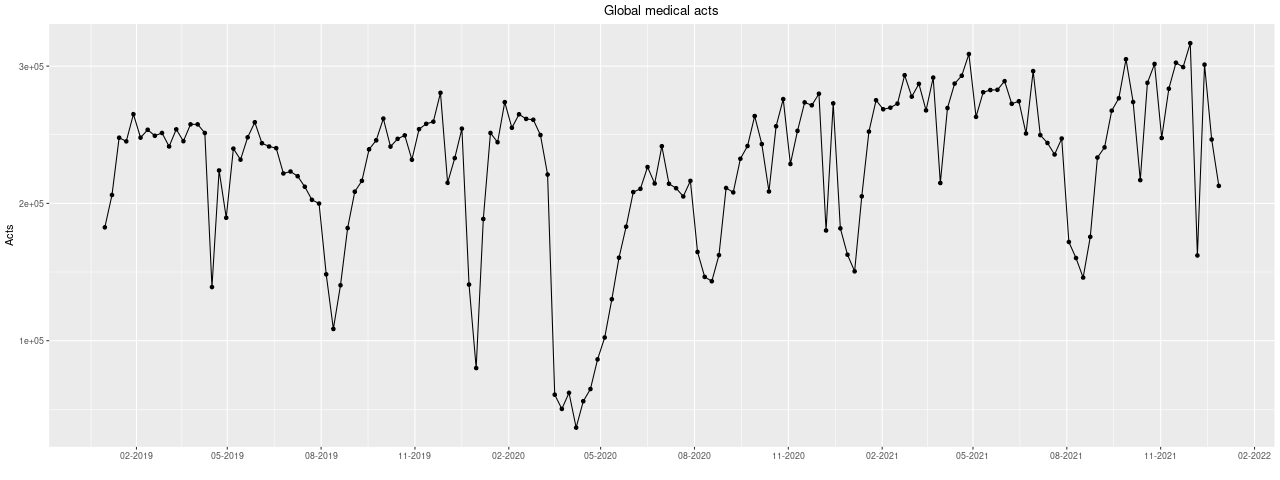
\includegraphics[width=8.0cm]{global_acts}
%          \Ovalbox{\vbox to 1.5in{\vfill\hbox{\vtop{\hsize=2.5in\hfill}\hfill}\vfill}}
%          \medskip
%          \centerline{(a)}
%        \end{minipage}\hfill
%        \begin{minipage}[t]{0.3\linewidth}\centering
%          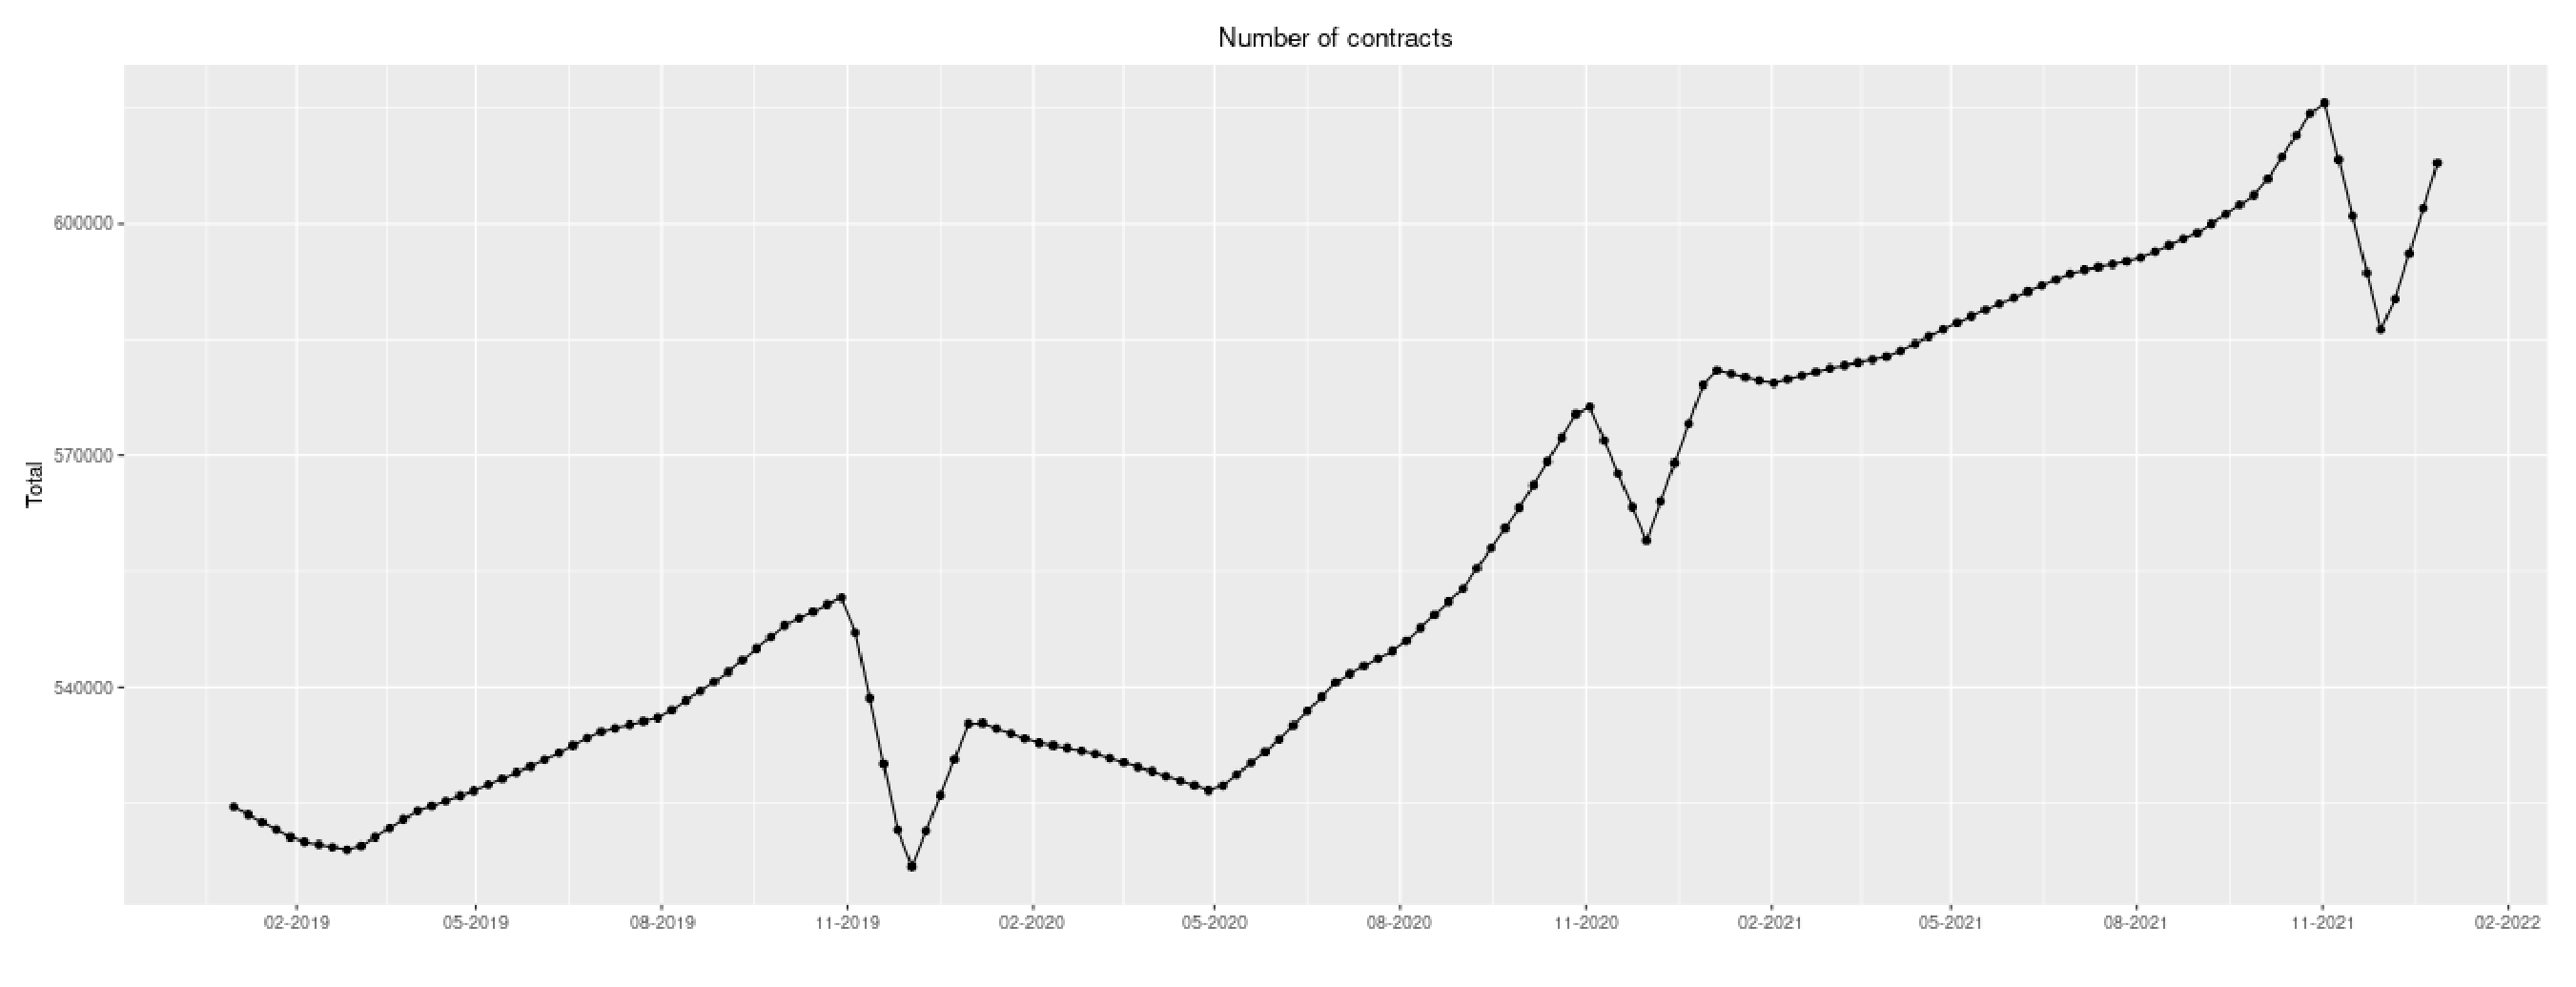
\includegraphics[width=8.0cm]{global_contracts}
%          \Ovalbox{\vbox to 1.5in{\vfill\hbox{\vtop{\hsize=2.5in\hfill}\hfill}\vfill}}
%          \medskip
%          \centerline{(b)}
%        \end{minipage}\hfill  
%        \begin{minipage}[t]{0.3\linewidth}\centering
%                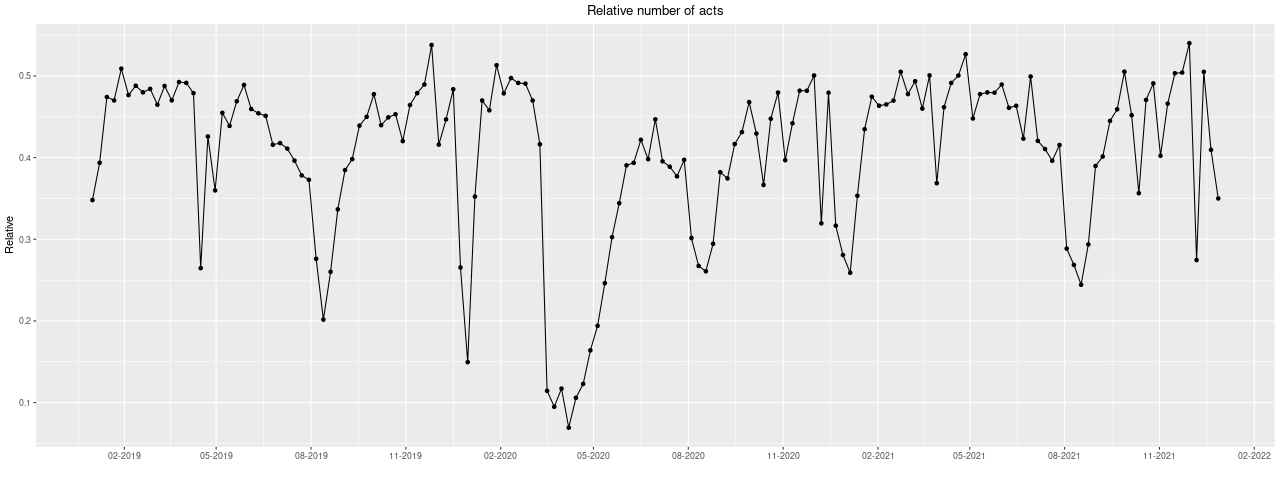
\includegraphics[width=8.0cm]{global_relative}
%                \Ovalbox{\vbox to 1.5in{\vfill\hbox{\vtop{\hsize=2.5in\hfill}\hfill}\vfill}}
%                \medskip
%                \centerline{(c)}
%              \end{minipage}\hfill
%          \caption{(a): Número semanal global de actos médicos entre Enero de 2019 y Diciembre de 2021; %(b): Número total de pólizas vigentes semanalmente entre Enereo de 2019 y Diciembre de 2021; (c): %Evolución del número total semanal de actos médicos relativo al total de pólizas vigentes entre Enero %de 2019 y Diciembre de 2021.}
%    \label{fig:1}
%\end{figure}       

%\section{Aplicación a actos médicos}

%Section with a figure (Fig.~\ref{fig:example}).


% Plots (PostScript files) are included through the ``figure'' environment.
% For more complicated figures use the minipage commaned (see LaTeX manual).
% --------------------------------------------------------------------------
\begin{figure}[H]

  \begin{minipage}[t]{1.0\linewidth}\centering
    %\Ovalbox{\vbox to 1.5in{\vfill\hbox{\vtop{\hsize=2.5in\hfill}\hfill}\vfill}}
    \centerline{\epsfig{figure=global_acts.eps,width=16.0cm}}
    \medskip
    \centerline{(a)}
  \end{minipage}\hfill

  \begin{minipage}[t]{1.0\linewidth}\centering
    \centerline{\epsfig{figure=global_contracts.eps,width=16.0cm}}
    %\Ovalbox{\vbox to 1.5in{\vfill\hbox{\vtop{\hsize=2.5in\hfill}\hfill}\vfill}}
    \medskip
    \centerline{(b)}
  \end{minipage}

  \bigskip

  \begin{minipage}[t]{1.0\linewidth}\centering
    \centerline{\epsfig{figure=global_relative.eps,width=16.0cm}}
    %\Ovalbox{\vbox to 1.5in{\vfill\hbox{\vtop{\hsize=2.5in\hfill}\hfill}\vfill}}
    \medskip
    \centerline{(c)}
  \end{minipage}\hfill

  %\begin{minipage}[t]{0.49\linewidth}\centering
  %  \centerline{\epsfig{figure=figures/regbsdcod.eps,width=8.0cm}}
  %  \Ovalbox{\vbox to 1.5in{\vfill\hbox{\vtop{\hsize=2.5in\hfill}\hfill}\vfill}}
  %  \medskip
  %  \centerline{(d)}
  %\end{minipage}

  \caption{Evolución temporal entre Enero de 2019 y Diciembre de 2021.}
  \label{fig:1}
\end{figure}

% Bibliography.
% -------------
\parskip=0pt
\parsep=0pt
\bibliographystyle{ieeetrsrt}

% Important: substitute your BiBTeX (*.bib) files below.
% ------------------------------------------------------
\bibliography{report}

\end{document}
